\begin{abstract}
Large language models now grade other language models, feeding leaderboards, reward models, and quality gates that all assume the writing system of an answer does not move its score. We test that assumption for Hindi, written natively in Devanagari and, by hundreds of millions online, in the Latin alphabet. We hold content fixed and vary only the script: 150 instruction-response pairs at three quality tiers, each in Devanagari and three romanizations (scholarly IAST, diacritic-stripped ASCII, user-style Hinglish), scored blind by seven judges from four families. An informal directional prediction, logged before data collection, said romanized text would score lower; the data mostly reversed it. First, Gemini 3.6 Flash scores identical romanized content \textbf{2.2 to 3.4 points higher} than Devanagari (all $p \le 0.003$), concentrating at \textbf{6.5 to 7.8 points} on medium-quality responses, where a judge has the most discretion; Gemini 3.1 Pro shows the same sign, smaller. Second, Qwen2.5-7B inflates IAST by \textbf{7.6} and ASCII by \textbf{6.0} points, reaching $\mathbf{+17.8}$ on low-quality items yet flat on Hinglish. Third, Claude judges move \emph{opposite}, the direction we pre-registered, and only on the lossy form: under a matched temperature-0 gateway Sonnet 5 penalises diacritic-stripped ASCII by \textbf{3.6} points ($p = 5\times10^{-5}$; $-9.2$ on high-quality items) while lossless IAST is null, a penalty that widens under the judge's default interface (a protocol variant, \S4.3) and replicates at full power on a same-size non-Claude-authored set ($-5.1$, $p = 2 \times 10^{-4}$; high tier $-16.6$); Opus 5 is smaller, Fable 5 near-invariant, GPT-5.6 near-robust. The inflation effects, by contrast, hold on the \emph{lossless} IAST transform itself (Flash $+3.4$, Qwen $+7.6$), so they cannot be artifacts of degraded text. Fourth, protocol decides what you see: batching alone erases the $-12.3$ ($\to +1.1$), and in pairwise trials \emph{all seven} judges prefer the Devanagari twin, six with zero ASCII wins in 300 trials each ($p<10^{-85}$), reversing even judges whose pointwise scores inflate ASCII. Fifth, prompting does not fix it: mitigation is at best partial on Gemini, flips sign under a rubric variant, and \emph{backfires} on Qwen (up to $+11.8$ from $+7.6$). A per-dimension decomposition shows Sonnet's penalty is 68 percent clarity but leaks significantly into correctness, which identical content cannot differ on; token length is ruled out ($|r|\le0.18$) while rationales name the orthography on 41 to 57 percent of romanized items. A Serbian Cyrillic/Latin replication on a lossless script pair finds the same discretion signature: overall shifts near zero, but both judges tested penalise Latin at the medium tier ($p \le 0.036$). Script effects in LLM judges are real, sign-opposite across families, protocol-sensitive in magnitude and sign, and not reliably promptable away.
\end{abstract}

\begin{figure}[t]
  \centering
  
\includegraphics[width=0.58\textwidth]{assets/fig1_schematic.png}
  \caption{\textbf{Study design.} One Hindi response, four orthographies, seven blind judges. Any score gap is script bias by construction; measured outcomes previewed at right (\S\ref{sec:results}).}
  \label{fig:schematic}
\end{figure}

\section{Introduction}

Evaluation of language models has largely been handed to other language models. An LLM judge reads a question and an answer and returns a score \citep{zheng2023judging} that then ranks systems on leaderboards, trains the next model as a reward signal, and gates what production systems ship. The reliability literature has catalogued many failure modes of these judges, including position bias \citep{wang2023fair}, verbosity and self-enhancement bias \citep{zheng2023judging}, self-preference driven by self-recognition \citep{panickssery2024self}, and taxonomies now spanning a dozen or more bias types \citep{ye2024justice, zhou2026judgebiasbench}. Every catalogue so far shares one silent assumption: that the \emph{writing system} of the judged text does not move the score.

That assumption matters most for languages with two written lives, and Hindi is the clearest case: its official script is Devanagari, but much of Hindi on phones and social media is typed in the Latin alphabet \citep{sheth2025comilingua}. The two forms carry identical content; a judge scoring them differently is measuring orthography, not quality.

This paper asks one narrow question with a clean design: hold the language and content of an answer fixed, change only its script, and ask whether an LLM judge's score moves. Because the content on both paths is identical (Figure~\ref{fig:schematic}), nothing else can explain a gap. Prior multilingual judge studies compared different languages, entangling language with script \citep{hada2024evaluators, fu2025reliable, zhou2026lower}; we untangle them.

We logged the predicted direction before collecting data: by analogy to the task-performance literature \citep{khullar2025scriptgap, rajapakse2026sinhala}, romanized text would score \emph{lower}. The data mostly reversed it: romanized Hindi scores \emph{higher} on Gemini and Qwen judges, the inflation concentrates where a judge has discretion, and it persists or worsens when the judge is told to ignore the script; Claude judges alone move in the predicted direction, and only in isolated judging. We report the reversal as found.

Our contributions:
\begin{itemize}
  \item \textbf{Script-controlled judge audit} (\S\ref{sec:method}): the first audit isolating script as a treatment: 150 fixed Hindi items, four orthographies, seven judges, four families, 21{,}204 scripted judgments (4{,}200 core, 600 matched-gateway core, 2{,}400 protocol arms, 7{,}200 mitigation-battery, 1{,}200 sub-dimension, 2{,}100 pairwise, 600 cross-script, 900 test-retest, 900 authorship-replication, 300 anchored, 300 ranking-demo, 204 Serbian).
  \item \textbf{A new, sign-opposite judge-bias axis} (\S\ref{sec:results}): up to $+7.8$ points of romanization inflation under Gemini 3.6 Flash and $+17.8$ under Qwen2.5-7B, against a Claude Sonnet 5 \emph{penalty} of $-3.6$ matched-gateway ($-12.3$ under its default interface); orthography appears in no existing judge-bias taxonomy \citep{ye2024justice, zhou2026judgebiasbench}.
  \item \textbf{A protocol effect that masks, and can even reverse, the bias} (\S\ref{sec:protocol}): a single-variable control shows batching alone erases Sonnet's $-12.3$ ASCII penalty, and pairwise judging flips Flash's pointwise inflation into near-total Devanagari preference (288/300 trials, zero ASCII wins), a warning for judge-bias audits and arena-style leaderboards alike.
  \item \textbf{A six-arm mitigation battery that fails in three different ways} (\S\ref{sec:mitigation}): prompting reduces the bias at best partially, flips its sign at worst, and amplifies it on the open-weights judge; the practitioner remedy is judge selection and script-stratified reporting, not prompting.
  \item \textbf{Mechanism probes} (\S\ref{sec:mechanism}): token length is ruled out as the driver, and the judges' rationales show the script is perceived while the miscalibration happens anyway.
\end{itemize}

\section{Related Work}
\label{sec:related}

\textbf{LLM-as-judge and its biases.} \citet{zheng2023judging} established the paradigm and catalogued position, verbosity, and self-enhancement biases; \citet{wang2023fair} flipped pairwise judgments by candidate order alone; \citet{panickssery2024self} traced self-preference to self-recognition; CALM \citep{ye2024justice} and JudgeBiasBench \citep{zhou2026judgebiasbench} quantify a dozen-plus bias types. Orthography is absent from all of these.

\textbf{Multilingual judging.} \citet{hada2024evaluators} calibrated GPT-4 judging against native speakers across eight languages, finding systematic overscoring, worst for low-resource languages; METAL \citep{hada2024metal} and PARIKSHA \citep{watts2024pariksha} measured judge-human agreement across languages; MM-Eval \citep{son2024mmeval} and \citet{fu2025reliable} stress-tested judges across up to 122 languages; BabelJudge \citep{kc2026babeljudge} measures Hindi reliability in native script only \citep[see also][]{zubiaga2026multilingualjudge}. Closest to us, \citet{zhou2026lower} audit 23 languages and note a Latin-script advantage observationally. In all of these, script co-varies with language; none isolates it.

\textbf{Script and romanization in LLMs.} RomanSetu \citep{husain2024romansetu} showed romanization can serve as an efficient adaptation interface for Indic languages, building on a longer transliteration-adaptation history \citep{purkayastha2023romanization, xhelili2024breaking, madhani2023aksharantar}. On deployment, Script Gap \citep{khullar2025scriptgap} measured task-accuracy drops up to 24 points on romanized inputs across five Indian languages, \citet{rajapakse2026sinhala} measured over 300-fold perplexity degradation on romanized Sinhala, and Indi-RomCoM \citep{das2026indiromcom} benchmarked romanized code-mixed degradation \citep[resources:][]{sheth2025comilingua, yang2025codemixbench}. Mechanistically, RomanLens \citep{saji2025romanlens} finds latent romanization inside multilingual models, and \citet{karne2026onelanguage} shows concept representations are not script-invariant. All of this measures the model as a task performer or probes its internals; none measures it as a judge.

\textbf{Tokenizer inequity.} Tokenizers price languages unequally \citep{petrov2023tokenizers, ahia2023costs, ali2024tokenizer, liang2023xlmv}; Indic byte-fallback fragmentation has been quantified as an eight-fold token tax \citep{srivastava2026tokenizertax}, with morphology-aware remedies proposed \citep{limisiewicz2024myte, brahma2025morphtok}. This literature stops at token counts and task accuracy; we test, and reject, its natural prediction for judge scores.

Much of the closest work is contemporaneous and not yet peer-reviewed (2026 preprints are marked in the references); we cite it for positioning, and no claim in this paper depends on any of it being correct.

\textbf{Indic evaluation.} Indic benchmarks evaluate in the conventional native script only \citep{ahuja2023mega, doddapaneni2023indicxtreme, singh2024indicgenbench, verma2024milu}; Airavata \citep{gala2024airavata} exemplifies current practice, its Hindi generations GPT-4-judged in Devanagari with the judge unvalidated. Our result says that practice is sensitive to an unexamined variable.

\section{Method}
\label{sec:method}

\textbf{Dataset.} We construct 150 Hindi instruction and response pairs (authored by a Claude-family model under human-specified tier definitions; \S\ref{sec:limitations} discusses the resulting self-preference exposure) across ten everyday domains, at three intended quality tiers of 50 items each: high (correct, complete, 80 to 140 words), medium (correct but visibly incomplete, 40 to 80 words), and low (curt, vague, or shallow, 15 to 40 words, a few with deliberate minor factual errors). Responses were authored in Devanagari and frozen before any judging. Tier intent was strongly realised: Devanagari means of 99.1, 51.4, and 15.2 under Gemini 3.6 Flash.

\textbf{Conditions.} Each frozen response is rendered in four orthographies. \emph{deva} is the original Devanagari. \emph{iast} is scholarly romanization with diacritics, produced deterministically with the indic-transliteration library \citep{madhani2023aksharantar}. \emph{ascii} strips the diacritics from IAST, a proxy for plain-keyboard romanization; the stripping is lossy (long/short vowel and retroflex/dental distinctions merge), which is precisely what plain-keyboard typing loses, so the ascii cell tests a degraded-but-ecological form while \emph{iast} tests a lossless one. \emph{hinglish} is a natural user-style respelling (for example \emph{kaise hain aap}), produced under a strict no-paraphrase rule: every word, the word order, and all punctuation preserved. In every condition the \emph{instruction} is rendered in the same orthography as the response (the ascii cell uses the IAST instruction), so a romanized response never answers a Devanagari question; \S\ref{sec:followup} also measures the deliberately mismatched cells. A native-speaker audit of a stratified 20-item sample of the hinglish condition confirmed 20/20 preserve content exactly; the audited sample ships with the released data.

\textbf{Judges and protocol.} Seven judges from four families score every item in every condition on a 0 to 100 rubric (correctness, completeness, helpfulness, clarity). Gemini 3.6 Flash and Gemini 3.1 Pro Preview are called through the API at temperature 0, one item per call, in randomized order, so the judge never sees two versions of the same item in one context. Claude Sonnet 5, Opus 5, and Fable 5 judge through blind agent sessions arranged in a Latin square: each session sees each item exactly once, in exactly one condition, with conditions rotated across four sessions. Qwen2.5-7B-Instruct runs open-weights under vLLM on one A10G GPU at temperature 0, one item per call, with top-20 logprobs recorded at the score position. GPT-5.6 is called one item per call at temperature 0 through a unified OpenAI-compatible gateway. No judge is told the study concerns scripts. The judging prompt asks for a score and a one-sentence reason; the reasons become data for the perception analysis (\S\ref{sec:mechanism}).

\textbf{Follow-up batteries.} Nine targeted batteries close the main alternative explanations (\S\ref{sec:followup}): a protocol control varying only batch size on a fixed interface; a per-dimension rubric decomposition on the main arms; an order-counterbalanced pairwise preference test; a cross-script control measuring the deliberately mismatched instruction/response cells; test-retest baselines for a deterministic and a stochastic judge; an anchored-pointwise variant with an in-context reference; a second-language replication in Serbian, whose Cyrillic-to-Latin transform is lossless; and Benjamini-Hochberg FDR correction plus a logit-scale tier reanalysis. Verbatim prompts and full tables are in the appendix.

\textbf{Analysis.} The unit of analysis is the within-item paired difference, romanized minus Devanagari, per judge and condition: mean shifts with bootstrap 95 percent CIs (10{,}000 resamples), two-sided sign-flip permutation tests (20{,}000 permutations), and paired $d_z$. Every number is produced by scripted analyses reading the raw score files; the outputs ship with the paper.

\textbf{Pre-registration.} Before data collection we recorded the predicted direction: romanized scores lower than Devanagari. The observed direction is mostly the opposite; we report all pre-specified analyses regardless.

\section{Results}
\label{sec:results}

\begin{table}[t]
\centering
\small
\caption{\textbf{Mean within-item score shift} (romanized minus Devanagari), bootstrap 95\% CIs, $n{=}150$. \textbf{Bold}: permutation $p<0.01$. One item per call throughout; the Sonnet (gateway) row is the temperature-0 matched-interface headline, the (CLI) row its default-sampling protocol variant (\S\ref{sec:followup}).}
\label{tab:main}
\begin{tabular}{lccc}
\toprule
Judge & IAST & ASCII & Hinglish \\
\midrule
Gemini 3.6 Flash & $\mathbf{+3.43}$ {\scriptsize$[+2.4, +4.6]$} & $\mathbf{+2.17}$ {\scriptsize$[+0.8, +3.7]$} & $\mathbf{+3.13}$ {\scriptsize$[+2.2, +4.1]$} \\
Gemini 3.1 Pro & $\mathbf{+1.17}$ {\scriptsize$[+0.6, +1.8]$} & $\mathbf{+1.10}$ {\scriptsize$[+0.4, +1.8]$} & $\mathbf{+1.13}$ {\scriptsize$[+0.5, +1.8]$} \\
Qwen2.5-7B & $\mathbf{+7.63}$ {\scriptsize$[+4.9, +10.4]$} & $\mathbf{+6.03}$ {\scriptsize$[+3.3, +8.7]$} & $+0.07$ {\scriptsize$[-1.8, +1.9]$} \\
Claude Sonnet 5 (gateway) & $+0.49$ {\scriptsize$[-0.6, +1.6]$} & $\mathbf{-3.64}$ {\scriptsize$[-5.0, -2.3]$} & $\mathbf{+1.89}$ {\scriptsize$[+0.9, +2.9]$} \\
Claude Sonnet 5 (CLI) & $\mathbf{-2.70}$ {\scriptsize$[-4.7, -0.8]$} & $\mathbf{-12.29}$ {\scriptsize$[-15.6, -9.2]$} & $\mathbf{-2.71}$ {\scriptsize$[-4.0, -1.4]$} \\
Claude Opus 5 & $-0.13$ {\scriptsize$[-0.8, +0.6]$} & $\mathbf{-3.43}$ {\scriptsize$[-4.4, -2.5]$} & $\mathbf{-1.18}$ {\scriptsize$[-1.9, -0.5]$} \\
Claude Fable 5 & $\mathbf{+1.43}$ {\scriptsize$[+1.0, +1.9]$} & $-0.30$ {\scriptsize$[-1.1, +0.4]$} & $+0.13$ {\scriptsize$[-0.3, +0.6]$} \\
GPT-5.6 & $+1.21$ {\scriptsize$[+0.2, +2.2]$} & $+0.51$ {\scriptsize$[-0.6, +1.7]$} & $+0.62$ {\scriptsize$[-0.2, +1.5]$} \\
\bottomrule
\end{tabular}
\end{table}

\begin{figure}[t]
  \centering
  
\includegraphics[width=0.53\textwidth]{assets/fig2_forest.png}
  \caption{\textbf{Score shift by judge and romanization}, 95\% bootstrap CIs, $n=150$. Right of the dashed zero line means romanized scored higher.}
  \label{fig:forest}
\end{figure}

\subsection{Three families, three bias profiles}

Table~\ref{tab:main} and Figure~\ref{fig:forest} are the study in one view. Gemini 3.6 Flash scores the same content higher when romanized: $+3.43$ for IAST ($p = 5 \times 10^{-5}$, $d_z = 0.49$), $+2.17$ for ASCII ($p = 0.003$), $+3.13$ for Hinglish ($p = 5 \times 10^{-5}$, $d_z = 0.52$); Gemini 3.1 Pro shows the same sign at one-third to one-half the size (all $p \le 0.003$).

The open-weights judge changes shape. Qwen2.5-7B inflates formal romanizations dramatically, $+7.63$ IAST and $+6.03$ ASCII, but is flat on natural Hinglish. Its inflation lives elsewhere too: low-quality items shift $+17.8$ (IAST) and $+17.4$ (ASCII), the small judge failing to recognise bad content dressed in diacritics, while Hinglish, plentiful in web data \citep{sheth2025comilingua}, is judged as soberly as Devanagari.

The Claude family moves in the opposite direction, the one we pre-registered. Our headline Sonnet number is the matched-gateway arm: $-3.64$ on ASCII at temperature 0 ($p = 5 \times 10^{-5}$), concentrated at $-9.24$ on high-quality items, IAST and Hinglish near zero; under its default headless interface the penalty widens to $-12.29$ on ASCII ($d_z = -0.62$) and appears on IAST and Hinglish too. Opus 5 shows the same sign at a fraction of the size ($-3.43$ on ASCII, $-1.18$ on Hinglish), and Fable 5 is near-invariant, with one small inflation on IAST ($+1.43$). Within one family the penalty shrinks with presumed model scale, and the pattern extends across families: GPT-5.6 is likewise near-robust (largest shift $+1.21$ on IAST, $p=0.02$; ASCII and Hinglish indistinguishable from zero), though it still inflates low-tier romanized items by $+3.1$ to $+3.8$. Sonnet's rationales say why out loud: they call romanized responses ``awkward IAST-transliterated Hindi rather than natural Devanagari,'' treating the orthography itself as a quality defect. Because our rubric asks for a clarity sub-score, and stripped ASCII is plausibly less clear to a competent Hindi reader, part of the Sonnet penalty could be a legitimate clarity judgment; a per-dimension decomposition (\S\ref{sec:followup}) confirms clarity carries 68 percent of it but shows a significant residue on correctness and helpfulness, dimensions identical content cannot differ on.

Three conclusions follow. Script effects exist in both directions: the same romanized answer is overpaid by one family and taxed by another. They are properties of the judge, not the task. And they split by transform lossiness: the inflations hold on lossless IAST itself, while the Claude penalty concentrates on lossy ASCII, the ecological plain-keyboard form.

\begin{figure}[t]
  \centering
  
\includegraphics[width=0.57\textwidth]{assets/fig3_tiers.png}
  \caption{\textbf{Shift by quality tier}, Gemini judges, 95\% bootstrap intervals, $n=50$ per tier. High/low tiers sit near the score ceiling/floor.}
  \label{fig:tiers}
\end{figure}

\subsection{The bias lives where the judge has discretion}

Figure~\ref{fig:tiers} splits the shift by quality tier. Under Flash, high-quality items shift at most 1.3 points against a ceiling near 99, low-quality at most 2.7 against a floor near 15, while medium-quality items, near 51 in Devanagari, inflate by $+7.8$ (IAST), $+7.4$ (ASCII), and $+6.5$ (Hinglish), all $p \le 1.5 \times 10^{-4}$. The same shape holds for Pro at smaller magnitude. The medium tier is genuinely ambiguous, not merely mid-scored: the seven judges agree strongly on Devanagari quality overall (mean pairwise $r = 0.94$, minimum $0.82$), yet their per-item disagreement doubles exactly there (mean across-judge SD $13.8$ versus $6.6$ high and $8.0$ low). This is the pattern one expects if romanization blurs the judge's view of quality: content whose flaws are obvious stays low, content whose merits are obvious stays high, and ambiguous content drifts toward a generous middle. It is also the pattern a purely mechanical ceiling-and-floor compression would produce with no discretion story at all; a logit-scale reanalysis (\S\ref{sec:followup}), which removes exactly that compression, still finds the medium tier's shift largest, so the discretion reading survives the transform. Appendix Figure~\ref{fig:example} shows one such drift verbatim: one refrigerator explanation, four orthographies, a thirty-point spread under one judge.

\subsection{The measurement protocol can hide the bias}
\label{sec:protocol}

\begin{figure}[t]
  \centering
  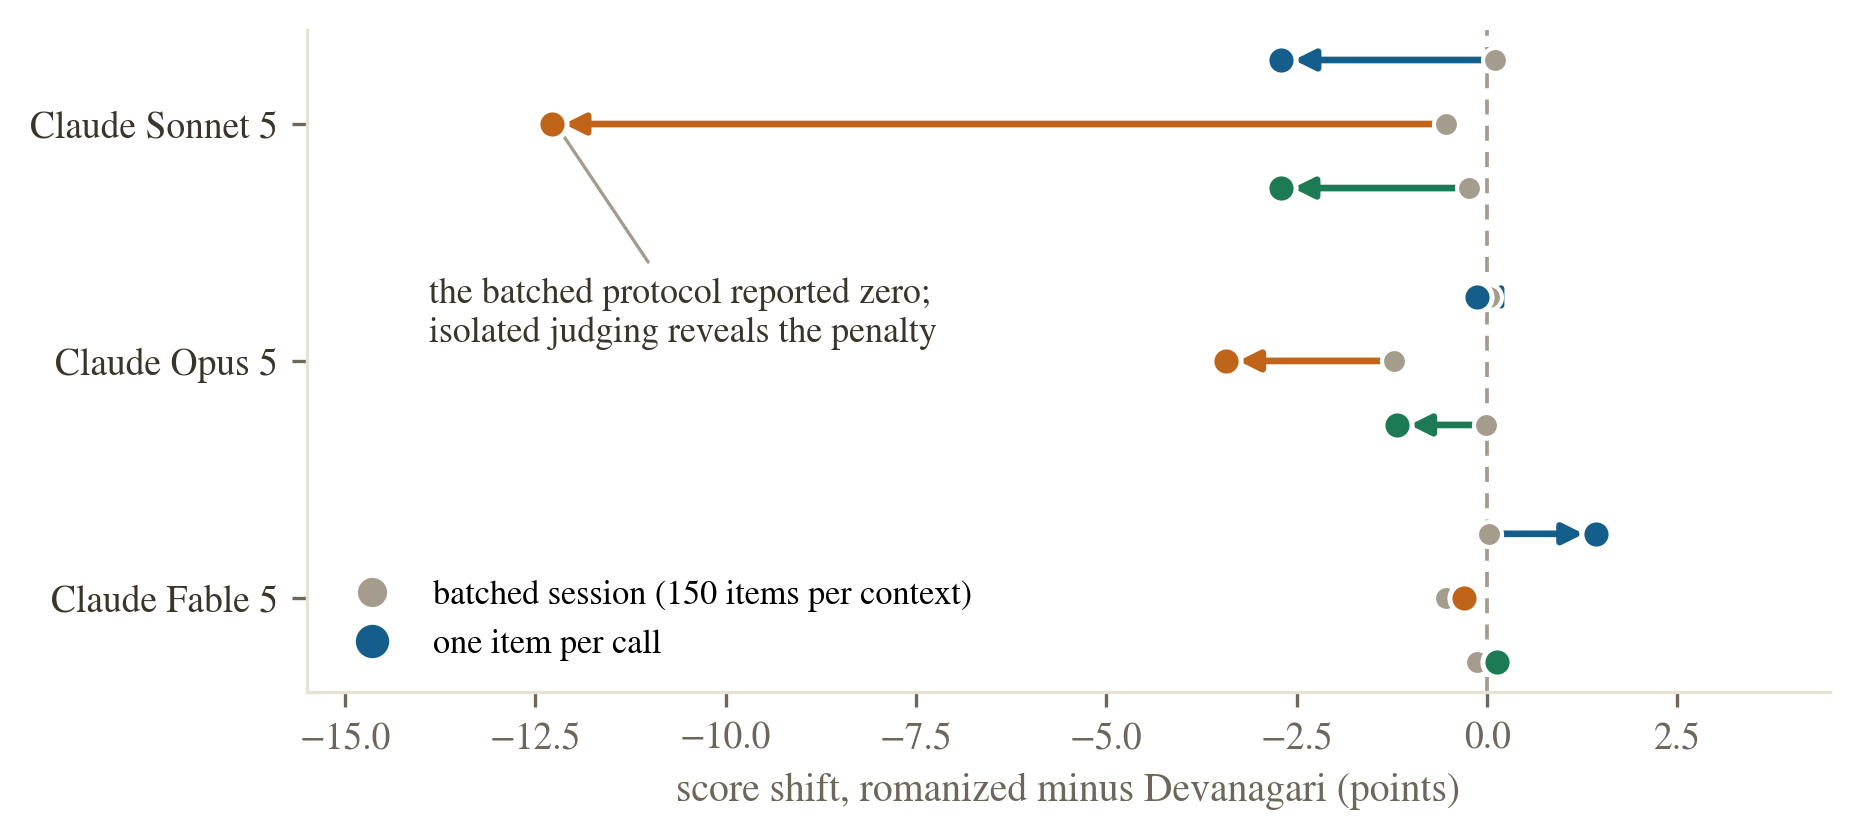
\includegraphics[width=0.52\textwidth]{assets/fig7_protocol.png}
  \caption{\textbf{Two protocols, two answers.} Batched sessions (grey) versus one item per call (colored) for the same three Claude judges; batching reports near-zero, isolation reveals penalties up to $-12.3$.}
  \label{fig:protocol}
\end{figure}

Our first Claude measurements used batched agent sessions, 150 items per context with conditions rotated in a Latin square; all three Claude judges appeared script-invariant, shifting at most 0.54 points in eight of nine comparisons. Rerunning the identical items one per call flipped the answer (Figure~\ref{fig:protocol}): the invariance was a batch artifact. Because those two arms also differed in interface and decoding temperature, we ran a single-variable control: the same Sonnet 5, the same headless interface, the same per-item rubric and sampling, with items grouped 25 per call. Batch size alone reproduces the masking: the $-12.29$ ASCII penalty becomes $+1.12$, and the high-tier penalty collapses from $-24.3$ to $-3.6$ (full table in the appendix). A judge that has just scored dozens of items appears to anchor its scale on content quality and stops reacting to surface form; in isolation, the orthography moves the score. Anchoring does not explain everything: batching also flips the IAST shift's sign ($-2.70 \to +2.64$), which masking alone cannot produce, so the batch context changes the judgment, not merely dampens it. Batched audits, common because they are cheap, can therefore mask, or invert, a bias production one-per-call judging would feel in full.

\subsection{Prompting does not reliably fix it}
\label{sec:mitigation}

The remedy every practitioner would try first is a line in the judge prompt. We tested six: a plain instruction, an explicit warning naming both scripts, a fairness framing, a transliterate-first instruction, a script-blind persona, and a decomposed rubric forcing four sub-scores summing to 100; each ran over the full four-condition protocol on two judge families (Appendix Figure~\ref{fig:mitigation}).

On Gemini 3.6 Flash, no arm closes the gap, though two help: transliterate-first cuts medium-tier inflation from $+7.8$ to $+4.4$, and the decomposed rubric more than halves the IAST and Hinglish shifts, but it overshoots on ASCII, flipping $+7.4$ to $-2.8$, trading inflation for penalty; the persona arm does nothing ($+7.7$). On Qwen2.5-7B the battery \emph{backfires} uniformly: every instruction increases IAST inflation above the $+7.6$ no-instruction baseline, up to $+11.8$ under the fairness framing, and the script-blind persona even induces a $+4.6$ Hinglish inflation where the baseline judge was flat. Mentioning scripts in the prompt appears to direct the smaller judge's attention to the very feature it should ignore. Prompt-level mitigation is therefore unreliable in the strongest sense: its effect ranges from partial reduction through sign reversal to amplification, consistent with debiasing results showing prompt-level fixes underperform training-level ones \citep{zhou2026judgebiasbench}. The practitioner remedy remains judge selection and script-stratified reporting, not prompting. The mitigation battery tests pointwise absolute scoring; whether these instructions transfer to pairwise preference judging is untested, and \S\ref{sec:followup} shows the pairwise protocol itself behaves very differently.

\subsection{Mechanism: not token length; the script is perceived}
\label{sec:mechanism}

Two probes narrow the explanation space. First, tokenization: the fairness literature predicts length disparities drive behaviour \citep{petrov2023tokenizers, ahia2023costs, srivastava2026tokenizertax}. Measured with the Gemini tokenizer, romanized Hindi is the \emph{expensive} form, 1.98 (IAST), 1.47 (ASCII), and 1.33 (Hinglish) times the Devanagari tokens (Appendix Figure~\ref{fig:mechanism}, left), reversing the romanization-efficiency premise of token \emph{savings} \citep{husain2024romansetu, brahma2025morphtok}. But token inflation does not explain the score inflation: the per-item correlation between token ratio and score shift is $r = +0.11$ (IAST), $+0.05$ (ASCII), and $-0.08$ (Hinglish), and no tier-restricted correlation exceeds $|r| = 0.18$. Longer input is not what earns the higher score. The top-20 logprobs recorded at the Qwen score position offer a partial distributional view: because they were captured at the first generated token only, they describe the leading digit of the score, not the full 0-100 value. On that limited view, romanized conditions shift the leading-token expectation upward (IAST $6.33$ versus Devanagari $5.70$) with essentially unchanged within-call spread, consistent with a mode move rather than a widening; a full-sequence distributional analysis remains future work.

Second, perception (Appendix Figure~\ref{fig:mechanism}, right): under Flash, 47/57/41 percent of IAST/ASCII/Hinglish rationales explicitly mention the script, against 1 percent for Devanagari; some name the orthography as a deficiency while scoring the item \emph{above} its Devanagari twin. The effect operates despite awareness, echoing the finding that internal representations are not script-invariant \citep{karne2026onelanguage, saji2025romanlens}.

\subsection{Follow-up batteries: closing the confounds}
\label{sec:followup}

Eight targeted batteries (4{,}500 judgments beyond the original 12{,}600: 600 GPT core and 600 batched control, already included in the core and protocol categories of \S\ref{sec:method}'s total, plus 1{,}200 sub-dimension, 600 pairwise, 600 cross-script, 600 test-retest, and 300 anchored; tables in the appendix) address the main alternative explanations.

\textbf{Noise floor.} Thirty stratified items, deva and ascii, five identical calls each, three judge families: mean within-item standard deviation is $1.66$ (Flash, temperature 0), $2.00$ (Sonnet, default sampling), and $2.58$ (GPT-5.6, temperature 0 via gateway). Sonnet's $-12.3$, Qwen's $+6.0$ to $+7.6$, and the medium-tier inflations sit five to seven of these standard deviations out; shifts near $\pm 1$ do not.

\textbf{Is the penalty just clarity?} Under the decomposed rubric, Sonnet's ASCII shift totals $-7.14$: clarity carries 68 percent, but correctness drops $-1.57$ ($p = 5 \times 10^{-5}$) and helpfulness $-0.54$ ($p = 0.001$), dimensions identical content cannot differ on. Flash's shift is pure clarity ($-2.29$). The non-clarity residue is bias by construction.

\textbf{Is it the interface?} Rerunning the full Sonnet arm through GPT-5.6's gateway at temperature 0, the ASCII penalty replicates in direction and tier structure at reduced magnitude ($-3.64$, $p = 5 \times 10^{-5}$; high tier $-9.24$), while the small IAST and Hinglish penalties do not ($+0.49$, $p = 0.40$; $+1.89$). The sign reversal against Gemini is interface-robust; the magnitude, like everything else here, is protocol-sensitive.

\textbf{Is it self-preference?} The 150 core items were Claude-authored (\S\ref{sec:limitations}), so we authored a same-size 150-item replication set with Gemini 3.1 Pro and reran both key judges at full power. Everything replicates on items no Claude model wrote: Sonnet's ASCII penalty ($-5.08$, CI $[-7.5, -2.5]$, $p = 2 \times 10^{-4}$; high tier $-16.64$, $p < 10^{-4}$) and Flash's inflation ($+5.27$ IAST, $+2.63$ ASCII, both $p \le 0.001$). Self-recognition cannot explain a penalty on another family's text.

\textbf{Is it question-answer script mismatch?} No: an ASCII response answering a \emph{Devanagari} instruction scores $13.5$ (Flash) and $16.1$ (Sonnet) points below the same response with a script-matched instruction (both $p = 5 \times 10^{-5}$), so mismatch is a separate, larger penalty that every headline number excludes by construction (\S\ref{sec:method}).

\textbf{Does pairwise judging agree?} No, starkly, and unanimously: shown the deva and ascii twins in both orders, every one of the seven judges prefers Devanagari (Flash 288/300, Sonnet 293/300, Pro 299/300, Opus and Fable 300/300, GPT-5.6 283/300, Qwen 252/300; all sign-test $p < 10^{-63}$). Qwen's graded pattern (8 ASCII wins, 40 ties) shows the format can produce ties and ASCII wins, ruling out a degenerate-prompt artifact; the capable judges simply never choose ASCII. Flash \emph{inflates} ASCII by $+2.2$ pointwise yet prefers Devanagari 96 percent of the time pairwise: the two standard protocols disagree not in degree but in sign, and preference-trained reward models sit on the pairwise side. An anchored-pointwise variant (the frozen Devanagari original as an in-context reference) points the same way: the ASCII inflation vanishes ($-0.97$, $p = 0.65$) and reverses to $-10.4$ on high-quality items, suggesting the pairwise verdict is the anchored assessment and unanchored pointwise is the outlier; the deva cell's response equals its reference, so this is directional evidence only.

\textbf{Does any of this survive a second language?} A 51-item Serbian set (Gemini-authored, same tiers) rendered in Cyrillic and Gaj Latin, an official transform lossless in both directions, shows small overall shifts (Flash $-1.08$, $p = 0.21$; Sonnet $-1.51$, $p = 0.11$), consistent with Latin Serbian's training abundance, but both judges independently penalise Latin exactly at the medium tier ($-3.82$, $p = 0.036$; $-4.76$, $p = 0.031$), high and low flat. The discretion signature travels across languages; overall size is language-dependent.

\textbf{Does a leaderboard actually move?} Three real systems (Qwen2.5-7B, Flash, Pro) answered 50 of our instructions in Hindi; Sonnet 5, a non-contestant, scored all 300 outputs in both scripts. The three-way ranking survives, but the script moves systems \emph{differentially}: Flash $-6.1$, Pro $-5.2$, Qwen $+2.8$ under romanization. These per-system shifts are the same order as the real Flash-Pro gap ($\approx 5$ points); no flip occurred in this triple, and whether closely matched systems actually swap remains untested.

\textbf{Multiple comparisons and scale artifacts.} Benjamini-Hochberg correction over all 198 reported p-values leaves 108 significant at $q = 0.05$ (effective threshold $p \le 0.0249$), including every headline effect. A logit-transform reanalysis of the tier pattern, which removes ceiling-and-floor compression, still places the largest shift at the medium tier for all three romanizations, so the discretion account survives (\S\ref{sec:results}).

\section{Limitations, narrated}
\label{sec:limitations}



There is no human reference score anywhere in this study. Every headline number is a shift relative to Devanagari, an anchor choice rather than validated ground truth: the data equally support judges under-scoring Devanagari, and words like ``inflates'' and ``penalises'' assert a direction of error the design cannot establish; read them as shorthand for ``shifts relative to Devanagari'' pending a human-anchored replication. The decomposition (\S\ref{sec:followup}) bounds the related clarity concern but cannot say whether the clarity component matches what a human reader experiences.

The dataset is model-authored and frozen; model-authored Hindi may differ from human Hindi in ways that interact with romanization. The hinglish condition is a model respelling under a strict no-paraphrase rule; a native-speaker audit of a stratified 20-item sample confirmed 20/20 preserve content, word order, and punctuation exactly, though it covers only hinglish and does not certify representativeness.

The Claude judges were measured under two protocols: batched agent sessions and headless one-item-per-call calls to the pinned model ids, the latter using default sampling where the API arms pin temperature 0. The batching control attributes the masking to batch size alone, and the matched-gateway arm (\S\ref{sec:followup}) now shows the Gemini-versus-Sonnet ASCII sign reversal survives on one interface at temperature 0; but the magnitude gap between the two Sonnet arms ($-12.3$ versus $-3.6$) is itself unexplained variance a fuller interface study should decompose. The 150 items were authored by a Claude-family model, so a self-recognition account \citep{panickssery2024self} initially predicted the Claude judges' preference for the authored surface form. The Gemini-authored replication set (\S\ref{sec:followup}) now excludes this for the headline effect: the high-tier ASCII penalty survives on another family's text. Smaller Claude-direction effects retain the exposure, and the full 150-item set remains single-authored.

The core arms ran one seed per item per condition; the test-retest batteries provide noise yardsticks that the headline effects clear several-fold, but per-item shifts near a point are indistinguishable from noise. The ranking demo shows differential per-system shifts of leaderboard-relevant size, but an observed flip between closely matched systems remains undemonstrated. Individual small cells that fail FDR (90 of 198 tests) should be read as unconfirmed.

Scale and scope are modest: one primary language plus a 51-item Serbian replication on two judges, 150 core items, seven judges, six prompt-level mitigation arms on two families, no training-level intervention. The quality tiers are coarse; the logit reanalysis (\S\ref{sec:followup}) defends the discretion account against scale compression, but a continuous-quality design would test it more sharply. The capability ordering rests on four checkpoints across two families with no independent capability metric: suggestive, not a scaling law. Extending to other digraphic settings \citep{karne2026onelanguage, rajapakse2026sinhala} is the natural next step.

Finally, the pre-registration was directional and informal (a project-log entry, not a registry filing); we state it because it disciplined our reporting of a reversed prediction.

\section{Conclusion}

We held Hindi content fixed, changed only its writing system, and asked seven LLM judges to grade it. The writing system moved the grades, in both directions: Gemini judges inflate romanized Hindi by 2 to 3 points overall and 7 to 8 on ambiguous-quality content; a 7B open-weights judge inflates formal romanizations by up to 18 points on low-quality content; Claude judges tax romanization instead, up to 12.3 points at the smallest scale in a suggestive capability ordering, while GPT-5.6 is near-robust; batch size alone erases the largest penalty; the judge that inflates ASCII pointwise prefers Devanagari in 96 percent of pairwise trials; the penalty is majority clarity but leaks into correctness; six mitigations range from partial to counterproductive; token length explains none of it; and the rationales prove the script is seen. The axis is real, judge-dependent in size and sign, protocol-sensitive in both, and belongs in every judge-bias taxonomy \citep{ye2024justice, zhou2026judgebiasbench} and multilingual evaluation checklist \citep{hada2024evaluators, son2024mmeval}, though establishing \emph{judge error} rather than \emph{non-invariance} still requires a human anchor (\S\ref{sec:limitations}). Until judges are audited for script invariance, Hindi evaluations should report native-script and romanized slices separately, and should say which judge produced the numbers.

\subsubsection*{Reproducibility Statement}
All datasets, per-call score files, the scripted analysis, figure build scripts, and spend logs accompany this submission and will be released publicly upon acceptance. Every number in this paper traces to a single analysis script reading the raw judgment files, described in \S\ref{sec:method}. Total marginal compute cost of the study was under 6 US dollars of metered API spend plus roughly one GPU-hour on a single accelerator for the open-weights judge; Claude judging ran through a separate subscription-billed interface not captured in that figure.

\subsubsection*{LLM Usage Statement}
Large language models were used as the subjects of this study (the seven judges under audit) and as engineering assistants for writing analysis code, drafting figures, and copy-editing this manuscript. All experimental design, statistical choices, interpretation of results, and claims are the authors'; every number reported was checked against the scripted analysis output described in \S\ref{sec:method} before being written into the text.
